\documentclass{article}

\usepackage{graphicx}
\usepackage{tikz}
\usepackage{tikzsymbols}
\usetikzlibrary{calc,patterns,shapes.geometric}
\pagestyle{empty}
\usepackage[margin=0pt]{geometry}
\geometry{papersize={14in,12in}}

\def\centerarc[#1](#2)(#3:#4:#5){\draw[#1] ($(#2)+({#5*cos(#3)},{#5*sin(#3)})$) arc (#3:#4:#5);}

\begin{document}
	\begin{figure}
		\centering
		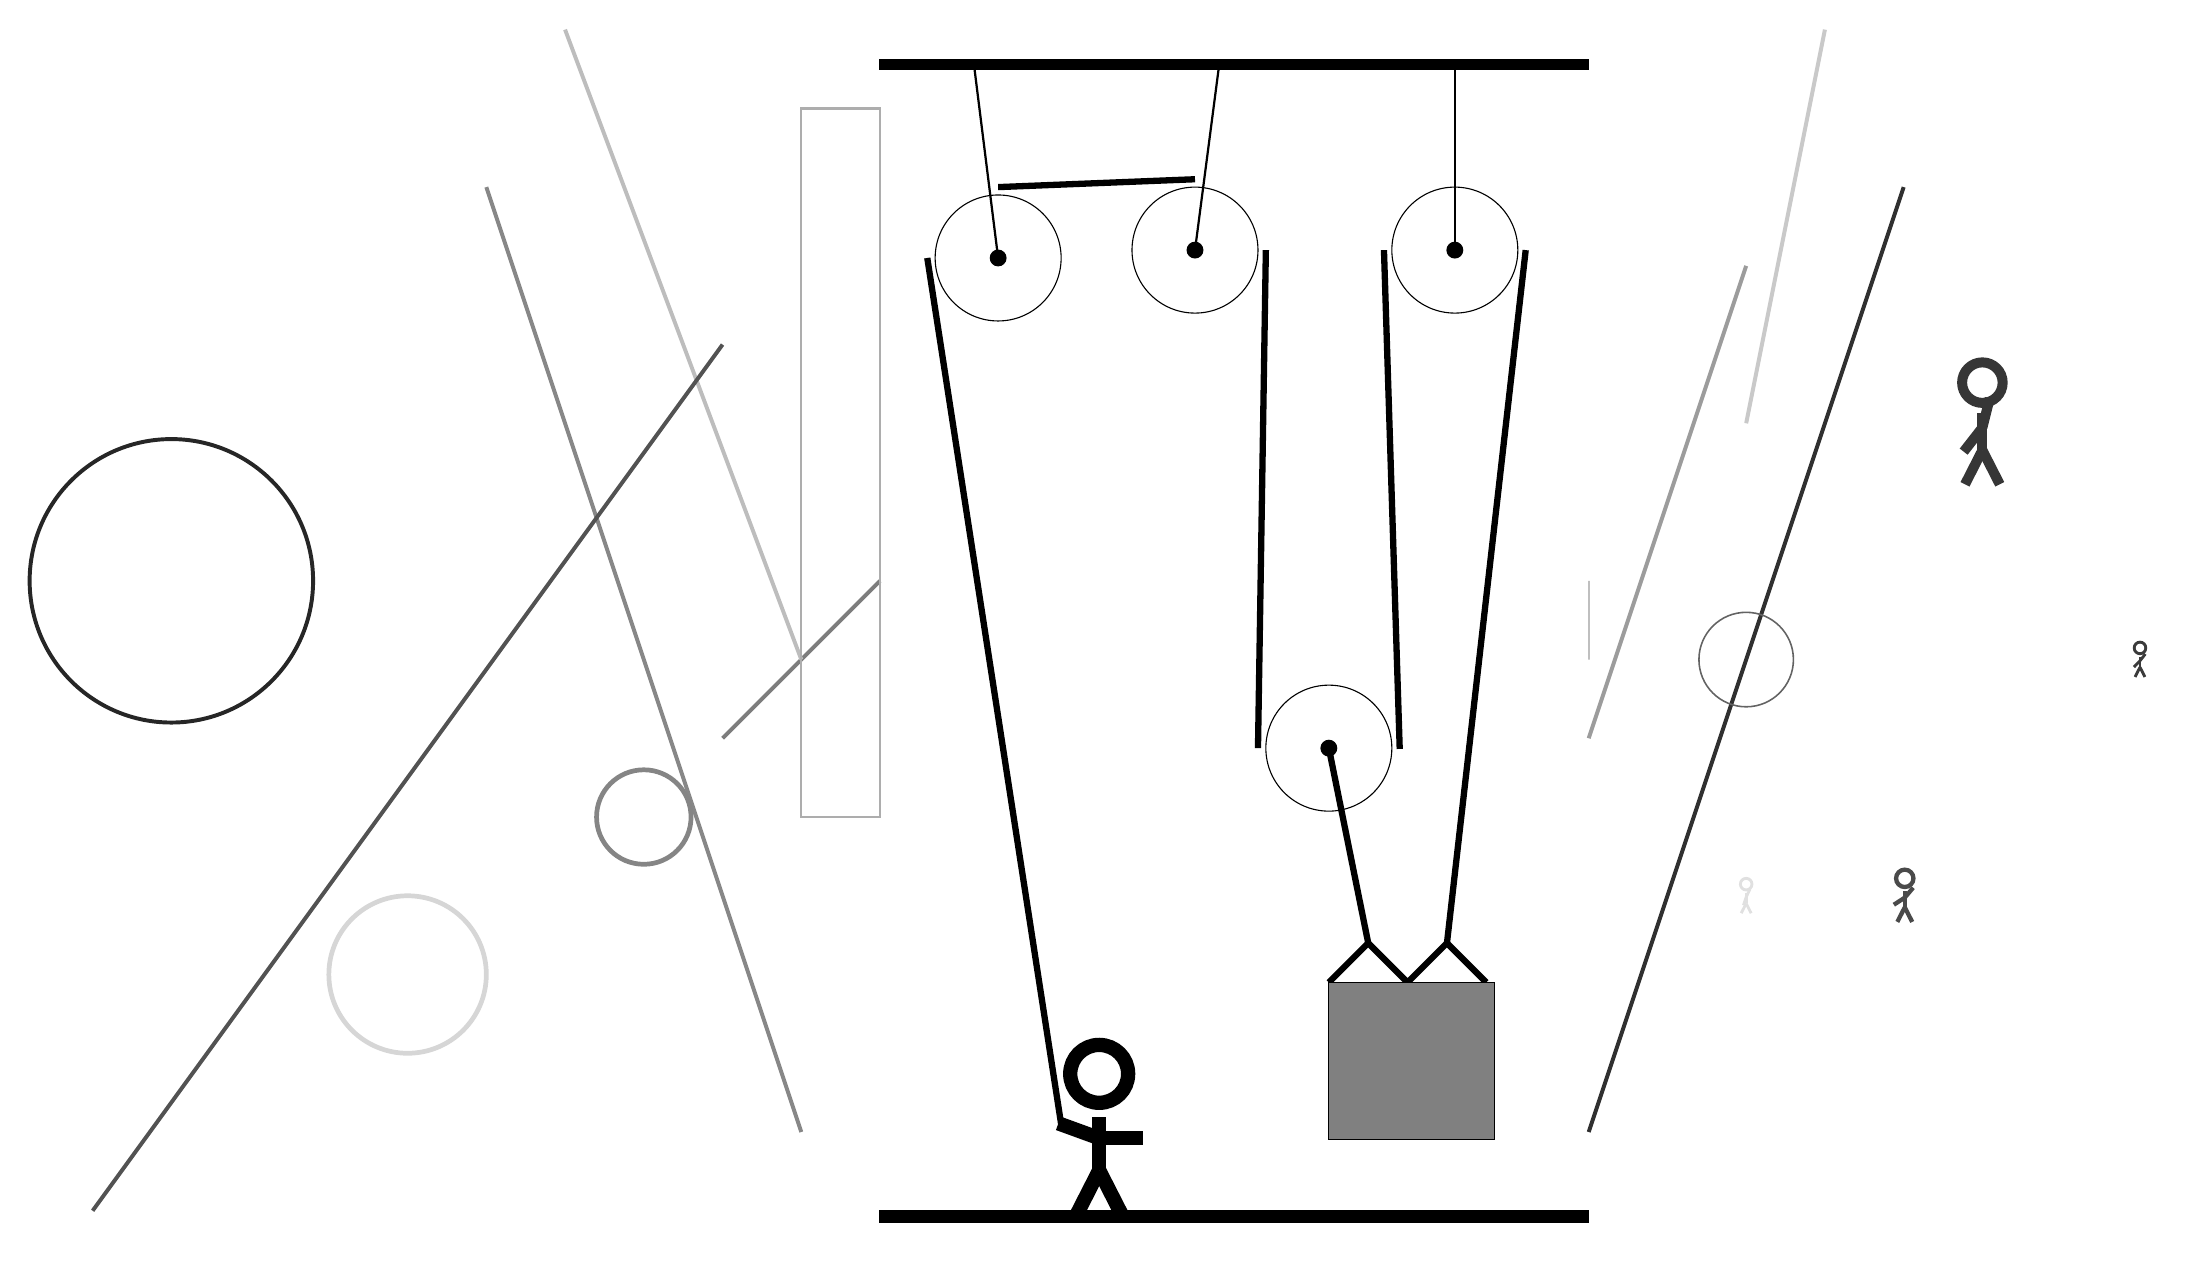
\begin{tikzpicture}
			%%%%% START %%%%%
			
			\draw[fill=black] (-3, 11.5) rectangle (6, 11.625);
			
			\draw (1, 9.2) circle (0.8);
			\draw[fill=black] (1, 9.2) circle (0.1);
			\draw[thick] (1, 9.2) -- (1.3, 11.5);
			
			\draw (4.3, 9.2) circle (0.8);
			\draw[fill=black] (4.3, 9.2) circle (0.1);
			\draw[thick] (4.3, 9.2) -- (4.3, 11.5);
			
			\draw (2.7, 2.875) circle (0.8);
			\draw[fill=black] (2.7, 2.875) circle (0.1);
			
			\draw[line width=0.8mm]  (2.7, -0.1) -- (3.2, 0.4) -- (3.7, -0.1) -- (4.2, 0.4) -- (4.7, -0.1);
			\draw[fill=black!50] (2.7, -0.1) rectangle (4.8, -2.1);
			
			\draw [line width=0.4mm, color=black!25](9, 2) circle (0.0);
			
			\draw[line width=0.5mm, color=black!51](-5, 3) -- (-3, 5);
			\draw[line width=0.5mm, color=black!47](-4, -2) -- (-8, 10);
			\draw [line width=0.5mm, color=black!85](-12, 5) circle (1.8);
			
			\draw [line width=0.6mm, color=black!48](-6, 2) circle (0.6);
			\draw[line width=0.5mm, color=black!26](-7, 12) -- (-4, 4);
			
			\draw[line width=0.5mm, color=black!39](8, 9) -- (6, 3);
			\node[line width=0.4mm, color=black!12] at (8, 1) {\Strichmaxerl[2][72][64]};
			\draw[line width=0.5mm, color=black!21](8, 7) -- (9, 12);
			\draw[line width=0.5mm, color=black!81](6, -2) -- (10, 10);
			
			\node[line width=0.5mm, color=black!77] at (13, 4) {\Strichmaxerl[2][46][52]};
			\draw[line width=0.5mm, color=black!68](-5, 8) -- (-13, -3);
			\node[line width=0.7mm, color=black!79] at (11, 7) {\Strichmaxerl[7][52][76]};
			
			\draw [line width=0.2mm, color=black!61](8, 4) circle (0.6);
			\draw [line width=0.6mm, color=black!16](-9, 0) circle (1.0);
			\node[line width=0.4mm, color=black!71] at (10, 1) {\Strichmaxerl[3][33][50]};
			\draw[line width=0.3mm, color=black!25] (6, 5) rectangle (6, 4);
			\draw[line width=0.3mm, color=black!32] (-3, 11) rectangle (-4, 2);
			
			\draw (-1.5, 9.1) circle (0.8);
			\draw[fill=black] (-1.5, 9.1) circle (0.1);
			\draw[thick] (-1.5, 9.1) -- (-1.8, 11.5);
			
			\draw[line width=0.8mm](-0.7, -1.9) --  (-2.4, 9.1);
			\centerarc[line width=0.8mm](-1.5, 9.1)(90:180:0.9);
			\draw[line width=0.8mm](-1.5, 10.0) -- (1, 10.1);
			\centerarc[line width=0.8mm](1, 9.2)(0:90:0.9);
			\draw[line width=0.8mm](1.9, 9.2) -- (1.8, 2.875);
			\centerarc[line width=0.8mm](2.7, 2.875)(180:370:0.9);
			\draw[line width=0.8mm] (3.6, 2.865) -- (3.4, 9.2);
			\centerarc[line width=0.8mm](4.3, 9.2)(0:180:0.9);
			\draw[line width=0.8mm](4.2, 0.4) -- (5.2, 9.2);
			\draw[line width=0.8mm] (3.2, 0.4) -- (2.7, 2.875);
			
			\node at (-0.2, -2) {\Strichmaxerl[10][-20][0]};
			
			\draw[fill=black] (-3, -3) rectangle (6, -3.15);
			
			%%%%% END %%%%%
		\end{tikzpicture}
	\end{figure}	
\end{document}